 
    Sparse linear algebra is central to many scientific codes, yet compilers
    fail to optimize it well.
    Instead, programmers rely on library implementations that are hand optimized
    and can utilize accelerator hardware.
    This comes at a cost, however, as it ties programs into vendor specific
    software ecosystems and results in non-portable code.

    This chapter develops an approach based on the {\em specification
    Language for implementers of Linear Algebra Computations} (LiLAC).
    Rather than requiring application developers to (re)write every program for
    a given library, the burden is shifted to a {\em one-off} description for
    the library implementer.
    The LiLAC-enabled compiler then uses this to incorporate library routines
    automatically.

    LiLAC provides automatic data marshaling, seamlessly maintaining state
    between calls as needed and minimizing data transfers.
    Appropriate places for library replacement are detected at the compiler
    intermediate representation level, making our approach language independent.

    We evaluate on legacy large-scale scientific applications written in FORTRAN;
    standard benchmarks written in C/C++ and FORTRAN; and C++ graph analytics kernels.
    Across heterogeneous platforms, applications and data sets we show performance
    improvements of 1.1x to over 10x without any user intervention.


\section{Introduction}

    Linear algebra is an important component of many compute intensive
    applications.
    While there are many compiler papers examining automatic optimization of
    dense linear algebra, sparse codes have received less attention. 
    Sparse algorithms are, however, increasingly important as the basis for
    graph algorithms and data analytics \cite{Kepner2015GraphsMA}.

Ideally, we would like compilers to automatically map dense and sparse-based
codes to heterogeneous compute platforms efficiently and with no user
intervention. However,  this has proven difficult.

Instead, we see the wide-scale provision of fast libraries
\cite{cusparse,clsparse,mkl}, often provided by hardware vendors themselves.
They provide excellent performance, but place the burden of code rewriting on
the application developer and are rarely portable across platforms.
Rewriting legacy applications involves considerable effort, especially when
using hardware accelerators that require careful data marshaling.
In fact, the difficulty of efficient integration is a key impediment to the
wider use of accelerator libraries.
Furthermore, source code modifications reduce the portability of the
program and require a commitment to specific hardware vendors, resulting in legacy
code bases that quickly become obsolete.

In this chapter, we reexamine the way that compilers and libraries are used
to tackle the challenge of achieving full performance without requiring any
application programmer effort.
Highly tuned and platform specific libraries are invariably the fastest
implementations available, therefore we use them as our building blocks.
We then develop a new specification language for implementers of such
libraries, the {\em specification Language for implementers of Linear Algebra
Computations} (LiLAC).

Using LiLAC, library implementers specify with a few lines of code,
{\em what} a library does and {\em how} it is invoked.  Our compiler
then determines where the library specification matches the user's
code and automatically rewrites the code to utilize library calls.

\paragraph*{LiLAC-What}
is a high level language to describe sparse and dense linear
algebra programs.
The LiLAC compiler uses it to detect such functionality
in user applications at the level of compiler intermediate representation.
It is powerful enough to formulate linear algebra, yet remains
independent of compiler internals and is easy to understand and program.

\paragraph*{LiLAC-How}
is a language to specify how parts of the LiLAC-What description
can be used for library invocations and how state can be retained in between
calls.
Our compiler uses this to automatically generate library call {\em harnesses} that
efficiently schedule memory transfers, execute setup code and handle hardware
context management.

Our approach is broadly applicable. To demonstrate its applicability
to legacy FORTRAN codes, we improved and extended the flang frontend
to LLVM and evaluated on a large-scale scientific application.
It also works on standard C/C++ and FORTRAN benchmark programs and C++ graph
\mbox{analytics} kernels. The presented LiLAC system achieves significant performance
improvement across heterogeneous platforms, from 1.1x to over 10x, without any
user intervention.

\begin{figure*}[t]
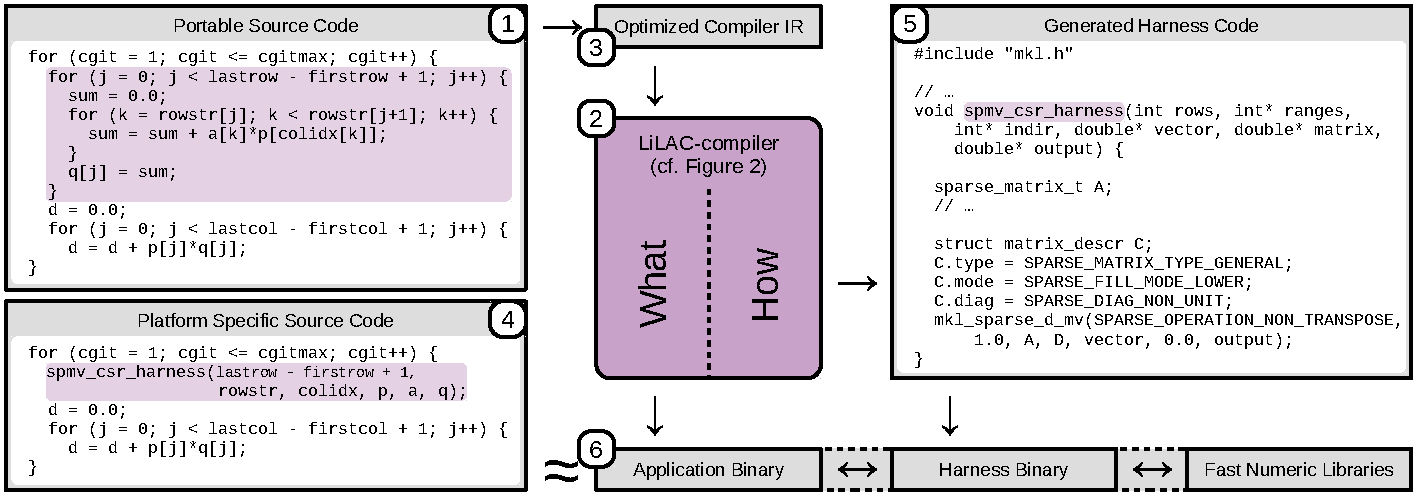
\includegraphics[width=\textwidth]{figures/lilac_overview.pdf}
\caption{LiLAC applied to NPB Conjugate Gradient:
         Code that matches the LiLAC-What specification is replaced with calls
         to a harness function. The harness is generated from a LiLAC-How
         specification to utilize Intel MKL.}
\label{motivationcode}
\end{figure*}

\section{Overview}
\label{sec:overview}

Consider the example in \autoref{motivationcode}.  In the top left
corner (1), we see unmodified application source code.  This is
{\em conjugate gradient} from the NAS-PB suite.  The program is written
in a straightforward manner and a naively compiled program would fail
to exploit the full potential of modern hardware.

In order to achieve good performance on Intel processors, we provide a
LiLAC specification of Intel MKL.
The LiLAC compiler (2) uses this to detect that the code in the framed loop is a
sparse matrix-vector product.
Instead of passing it on to the generic compiler backend, it replaces it with a
call to an auto-generated {\em harness} function  and captures the parameters of the computation
as function call arguments.
This is performed on optimized intermediate representation code (3)
and results in a program that is equivalent to the source code shown in the
bottom left (4).

LiLAC also automatically generates the corresponding harness as shown at
the right of the figure (5).
The resulting shared library is then linked with the application binary at
runtime, interfacing the underlying library implementation (6).

\begin{figure*}[t]
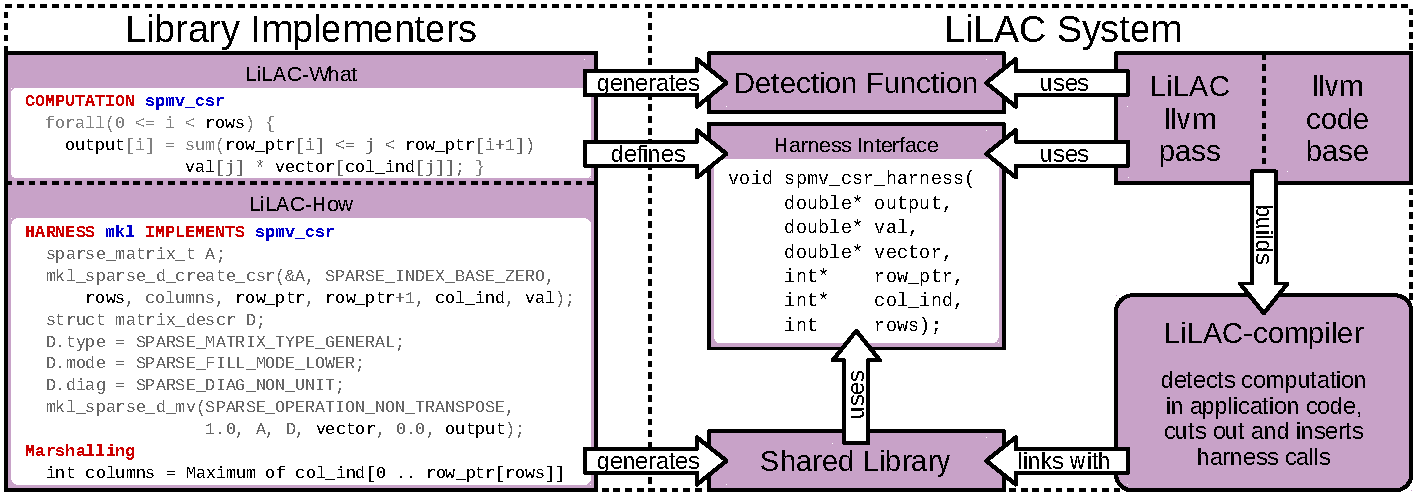
\includegraphics[width=\textwidth]{figures/whathowflow.pdf}
\caption{Overview of the LiLAC internals: On the left is the entire LiLAC
         program the library implementer must write. This results in a modified
         LiLAC-compiler in the bottom right that behaves as the shown in
         \autoref{motivationcode}.}
\label{motivationflow}
\end{figure*}

\subsection{Implementation Overview}

\autoref{motivationflow} provides more detail on the internals of
LiLAC.  On the left we can see the LiLAC specification provided by the
library implementer - just 16 lines of code.  It consists of a
{\em What} and a {\em How} part.  These two parts are processed by the
LiLAC system, eventually resulting in a runtime library and a modified
C/C++ compiler.

{\bf LiLAC-What} specifies the functionality that is provided by a library,
in this example {\em spmv-csr} (cf.\ \autoref{motivationcode}).
From this specification, a detection program that finds the computation in
normalized LLVM IR code is automatically generated and the harness interface
is determined.

{\bf LiLAC-How} specifies how the library, in this case Intel MKL, can be
invoked to perform the specified calculation.
This involves boilerplate code, but also advanced features, such as optimized
data transfers to accelerators.
In the last two lines, we can see how to efficiently compute the {\em columns}
variable with LiLAC.
It is not present in the {\em LiLAC-What} definition but is required by the MKL library. It  cannot be
captured statically and has to be computed at runtime using the values in the
{\em row\_ptr} array.
Using {\em Marshalling}, LiLAC automatically generates the harness
such that this is only recomputed if the values in {\em row\_ptr} change.

On the right of the figure we can see how the components generated from the
LiLAC specification are used to build the LiLAC-compiler.
Based on the LLVM infrastructure, it implements a transformation pass that
is executed after the normal optimization pipeline.
Using the generated detection function, it finds instances of the computation
and replaces them with calls to the specified harness interface.
Application binaries are dynamically linked to the harness library.

\section{What and How}

This section describes in more detail the two components of the LiLAC language.
LiLAC-What describes what a specific library does and LiLAC-How describes how
user code is bound to the underlying implementation.

\subsection{LiLAC-What: Functional Description}
At the heart of our approach is a simple language to specify sparse and dense
linear algebra operations.
This serves two purposes in our LiLAC system: Firstly, it is used to generate
a detection program for finding the computation in user code.
Secondly, it identifies the variables that are arguments to the library, thus
defining the harness interface.

The key challenge in the design of this language was to stay simple enough
to allow automatic generation of robust detection functionality, yet to be able
to capture interesting functionality.
Crucial for sparse linear algebra routines is capturing the many different
memory access patterns, the control flow on the other hand is very rigid.
This is reflected in the grammar as shown in \autoref{bnfgrammar}.

\subsection{Sparse Matrix Variations in LiLAC-What}
Sparse matrices can be stored in different formats.
In this section we introduce two of them and show how LiLAC-What can express
the corresponding computations.

\begin{figure}[t]
\begin{align*}
program ::=\ &\textbf{COMPUTATION} \left<name\right> \left<body\right>\\
body    ::=\ &\left<forall\right> \mid \left<dotop\right>\\
range   ::=\ &\textbf{(} \left<exp\right> \textbf{<=} \left<name\right> \textbf{<} \left<exp\right> \textbf{)}\\
forall ::=\ &\textbf{forall} \left<range\right> \textbf{\{} \left<body\right> \textbf{\}}\\
dotp    ::=\ &\left<addr\right> \textbf{=}\ \textbf{dot} \left<range\right> \left<addr\right> \textbf{*} \left<addr\right> \textbf{;}\\
addr    ::=\ &\left<name\right> \{\ \textbf{[} \left<exp\right> \textbf{]}\ \}\\
add     ::=\ &\left<exp\right> \textbf{+} \left<exp\right>\\
mul     ::=\ &\left<exp\right> \textbf{*} \left<exp\right>\\
exp     ::=\ &\left<name\right> \mid \left<cnst\right> \mid \left<addr\right> \mid\ \left<add\right> \mid \left<mul\right>
\end{align*}
\vspace{-1.5em}
\caption{Grammar of the LiLAC-What language}
\label{bnfgrammar}
\end{figure}

\begin{figure}[t]
\begin{minipage}[b]{0.3\linewidth}
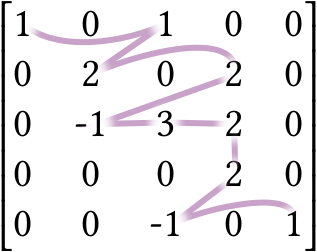
\includegraphics[width=0.9\linewidth]{figures/csrorder.png}
\vspace{0.04em}
\end{minipage}
\begin{minipage}[b]{0.65\linewidth}
\begin{align*}
\text{\bf val} =& \begin{bmatrix}
1\ \ 1\ \ 2\ \ 2\ \ \text{-}1\ \ 3\ \ 2\ \ 2\ \ \text{-}1\ \ 1\\
\end{bmatrix}\\
\text{\bf col\_ind} =& \begin{bmatrix}
0\ \ 2\ \ 1\ \ 3\ \ 1\ \ 2\ \ 3\ \ 3\ \ 2\ \ 4\\
\end{bmatrix}\\
\text{\bf row\_ptr} =& \begin{bmatrix}
0\ \ 2\ \ 4\ \ 7\ \ 8\ \ 10\\
\end{bmatrix}
\end{align*}
\end{minipage}
\caption{Compressed Sparse Row representation as used by the LiLAC-What example
         in \autoref{motivationcode}}
\label{csr_lilacwhat_fig}
\vspace{1.5em}
\centering
\begin{minipage}[b]{0.3\linewidth}
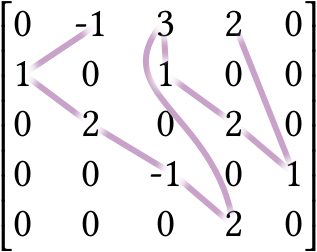
\includegraphics[width=0.9\linewidth]{figures/jdsorder.png}
\vspace{0.04em}
\end{minipage}
\begin{minipage}[b]{0.65\linewidth}
\footnotesize
\begin{align*}
\text{\bf perm} =& \begin{bmatrix}1\ \ 2\ \ 0\ \ 4\ \ 3\\\end{bmatrix}\\[-0.4em]
\text{\bf val} =& \begin{bmatrix}\text{-}1\ \ 1\ \ 2\ \ \text{-}1\ \ 2\ \ 3\ \ 1\ \ 2\ \ 1\ \ 2\\\end{bmatrix}\\[-0.4em]
\text{\bf col\_ind} =& \begin{bmatrix}1\ \ 0\ \ 1\ \ 2\ \ 3\ \ 2\ \ 2\ \ 3\ \ 4\ \ 3\\\end{bmatrix}\\[-0.4em]
\text{\bf jd\_ptr} =& \begin{bmatrix}0\ \ 5\ \ 9\ \ 10\\\end{bmatrix}\\[-0.4em]
\text{\bf nzcnt} =& \begin{bmatrix}3\ \ 2\ \ 2\ \ 2\ \ 1\end{bmatrix}
\end{align*}
\end{minipage}
\vspace{0.5em}
\hrule
\vspace{0.3em}
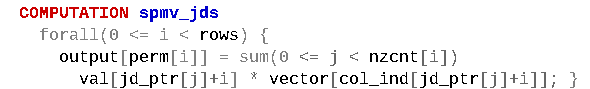
\includegraphics[width=\linewidth]{figures/spmvjdswhat.pdf}
\vspace{-1.2em}
\caption{Jagged Diagonal Storage in LiLAC-What}
\label{jds_lilacwhat_fig}
\end{figure}

\subsubsection{Compressed Sparse Row}
For Compressed Sparse Row (CSR) \cite{doi:10.1137/1.9780898718003}, all non-zero
entries are stored in a flat array \textbf{val}.
The \textbf{col\_ind} array stores the column position for each value.
Finally, the \textbf{row\_ptr} array stores the beginning of each row of the
matrix as an offset into the other two arrays.
The number of rows in the matrix is given directly by the length of the
\textbf{row\_ptr} array minus one, however the number of columns is not
explicitly stored.
In \autoref{csr_lilacwhat_fig}, a 5x5 matrix is shown represented in this
format, the LiLAC-What code is in the top left of \autoref{motivationflow}.

\subsubsection{Jagged Diagonal Storage}
For Jagged Diagonal Storage (JDS) \cite{doi:10.1137/0910073}, the rows of the
matrix are permuted such that the number of nonzeros  per row  decreases. The
permutation is stored in a vector \textbf{perm}, the number of nonzeros in
\textbf{nzcnt}.
The nonzero entries are then stored in an array \textbf{val} in the following
order: The first nonzero entry in each row, then the second nonzero entry in
each row etc.
The array \textbf{col\_ind} stores the column for each of the values and
\textbf{jd\_ptr} stores offsets into \textbf{val} and \textbf{col\_idx}.
The product of a sparse matrix in JDS format with a dense vector is specified 
in LiLAC-What at the bottom of \autoref{jds_lilacwhat_fig}.

\subsection{LiLAC-How}
\label{sec:lilachow}

    Where LiLAC-What specifies the computations that are implemented by a
    library, LiLAC-How describes how precisely library calls are to be be used
    for performing them.
    The langauge was designed with important existing libraries such as 
    cuSPARSE, clBLAS and Intel MKL in mind.
    In order to support the idiosyncrasies of these libraries, the
    specifications need to be built around boilerplate C++ code that manages the
    construction of parameter structures, calling conventions etc.
    However, it is also crucial for the specification language to be as
    high-level as as possible without sacrificing any performance, and the fine
    balance between these requirements drove the design of the language.
    In particular, LiLAC-How abstracts away memory transfers.

    The result is a language that can be further divided into two interacting
    components.
    Firstly, it describes boilerplate code that is required for individual library
    call invocations in a {\em harness}.
    Secondly, it is used for data {\em marshaling} between the core program and the
    library, which is particularly crucial for heterogeneous compute environments.
    \autoref{lilacbnf2} shows the grammar specification of LiLAC-How.

\subsubsection{Individual Library Invocations}
We need to encapsulate the boilerplate code that any given library requires,
such as setup code, filling of parameter structures etc.
This part of the language is straightforward.

\paragraph{Harness}
The harness construct is the central way of telling the LiLAC system how a
library can be used to perform a computation that was specified in LiLAC-What.
As we can see at the top of \autoref{lilacbnf2}, a harness refers to a
LiLAC-What program by name and also has a name itself.
It is built around some C++ code, which can use all the variables from the
LiLAC-What program to connect with the surrounding program.
It also needs to specify the relevant C++ header files
that the underlying library requires.
Lastly, the harness can incorporate persistent state and utilize data
marshaling functionality.

\paragraph{Persistence}
Many libraries need setup and cleanup code, which is specified with the
keywords {\em BeforeFirstExecution} and {\em AfterLastExecution}.
These are used in combination with {\em PersistentVariables}, allowing state to
persist between harness invocations, e.g.\ to retain handlers to hardware
accelerators.

\paragraph{Example}
In \autoref{mklharness1}, we see a trivial LiLAC-What program for implementing
\texttt{spmv\_csr} with the Intel MKL library.
The actual call to the relevant library function is in line 16.
To prepare for that call, there is boilerplate code in lines 7--14 to fill
parameter structures.

Critically, there is an additional parameter required by the library that is
not part of the LiLAC-What specification: the number of columns, {\em cols}, in
the sparse matrix.
It is determined at runtime, in lines 2--5, leading to reduced performance.
We will avoid this with the data marshaling constructs in the next section.

\subsubsection{Data Marshaling}
Heterogeneous accelerators require data transfers to keep memory consistent
between host device and accelerator.
To achieve the best performance, these have to be minimized.

Importantly, unchanged data should never be copied again.
This is not trivial to achieve, as it requires dynamic checks.
LiLAC-How uses hardware memory protection to implement this with minimal
run time overhead in generated harnesses.

\begin{figure}[t]
\centering
\begin{align*}
harness  ::=\ &\textbf{HARNESS} \left<name\right> \textbf{IMPLEMENTS} \left<name\right>\\[-0.3em]
              &\left<C++\right>\\[-0.3em]
           [\ &\left<marshalling\right>\ ]\ [\ \left<persistence\right> ]\\[-0.3em]
           [\ &\textbf{CppHeaderFiles}\ \{\ \left<name\right>\ \}\ ]\\
persistence ::=\ &\textbf{PersistentVariables}\ \{\ \left<name\right> \left<name\right>\ \}\\[-0.3em]
              [\ &\textbf{BeforeFirstExecution} \left<C++\right>\ ]\\[-0.3em]
              [\ &\textbf{AfterLastExecution} \left<C++\right>\ ]\\[-1em]
\cline{1-2}\\[-2em]
marshalling ::=\ &\textbf{Marshalling}\\[-0.3em]
          \{\ &\left<type\right> \left<name\right> \textbf{=} \left<name\right> \textbf{of}\\[-0.3em]
              &\left<name\right>\ \textbf{[}\ \textbf{0}\ \textbf{..} \left<exp\right> \textbf{]}\ \}\\
input   ::=\ &\textbf{INPUT} \left<name\right> \left<C++\right>\\[-0.3em]
             [\ &\textbf{BeforeFirstExecution} \left<C++\right>\ ]\\[-0.3em]
             [\ &\textbf{AfterLastExecution} \left<C++\right>\ ]\\
output  ::=\ &\textbf{OUTPUT} \left<name\right> \left<C++\right>\\[-0.3em]
             [\ &\textbf{BeforeFirstExecution} \left<C++\right>\ ]\\[-0.3em]
             [\ &\textbf{AfterLastExecution} \left<C++\right>\ ]
\end{align*}
\vspace{-1.5em}
\caption{Grammar of LiLAC-How}
\label{lilacbnf2}
\end{figure}

\begin{figure}[t]
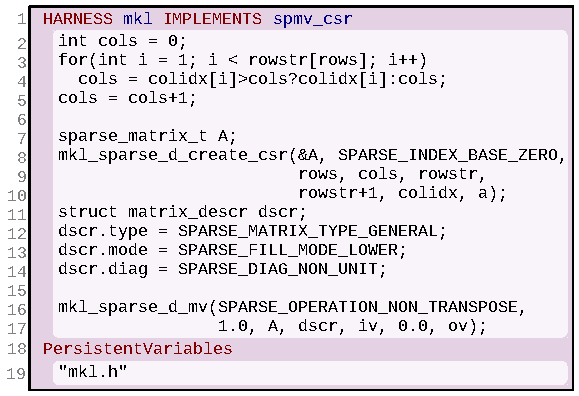
\includegraphics[width=0.944\linewidth]{figures/harness2.pdf}
\\[-0.75em]
\caption{This LiLAC-What code implements CSR SPMV na\"ively with Intel MKL.
         Performance is degraded because of lines 2--5.
         \autoref{readablemax} will present a solution to this bottleneck.}
\vspace{2.em}
\label{mklharness1}
\end{figure}

\begin{figure}[t]
\centering
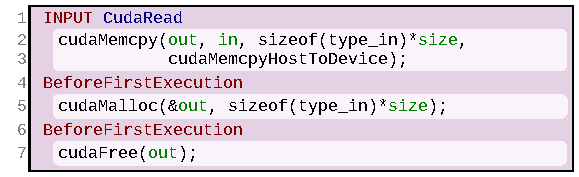
\includegraphics[width=0.944\linewidth]{figures/harness3.pdf}
\\[-0.75em]
\caption{LiLAC-How code to provide efficient automatic data marshaling between
         host and CUDA accelerator.}
\label{cudaread}
\end{figure}

\begin{figure}[t]
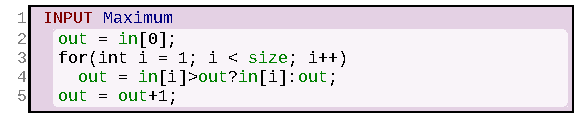
\includegraphics[width=0.944\linewidth]{figures/harness4.pdf}
\\[-0.75em]
\caption{{\em INPUT} can also be used to specify data dependent computations
         that are only recalculated when required.}
\vspace{0.5em}
\label{readablemax}
\end{figure}

\begin{figure}[t]
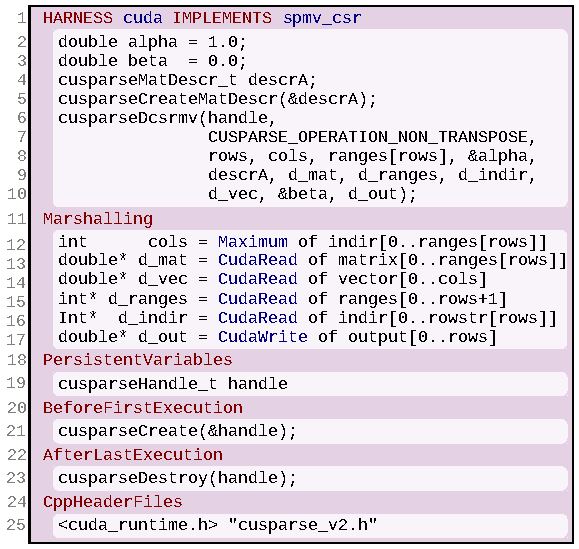
\includegraphics[width=0.944\linewidth]{figures/harness1.pdf}
\\[-0.75em]
\caption{This LiLAC-What specification implements an efficient SPMV harness
  using cuSPARSE in only 25 lines of code.}
\label{spmvharness}
\end{figure}

This data {\em marshaling} comes in two flavors; INPUT and OUTPUT.
Both of these are bound to a range of memory in the harness.
The LiLAC-generated code then uses hardware memory protection to detect read and
write accesses to these memory ranges.
In the specification, the underlying array is available using the
identifiers {\tt in}, {\tt size}, and {\tt out}.

\subsubsection{Detailed Example}
In \autoref{cudaread}, LiLAC-How functionality is specified using the
\texttt{cudaMemcpy} function from NVIDIA CUDA.
It is used to copy data from the host to the accelerator.
Note that for this to work, it first needs to allocate memory of the
device using \texttt{cudaMalloc}, which is later freed with \texttt{cudaFree}.
\texttt{cudaMemcpy} is executed only when a value in the array changes,
resulting in minimal memory transfers.

We can use the same construct to efficiently compute values
such as the \texttt{cols} variable in \autoref{mklharness1}, as shown in
\autoref{readablemax}.
The optimized implementation is nearly identical to the code in
\autoref{mklharness1} lines 2-5, however instead of the concrete variable name
the reserved identifiers {\tt in}, {\tt size}, and {\tt out} are used.
\pagebreak

We can now use these in \autoref{spmvharness}, showing a CSR SPMV
LiLAC-How program for the cuSPARSE library.
A number of data marshaling variables are introduced in lines 12--17, that
automatically optimize both memory transfers and the computation of the
\texttt{cols} variable.
The core of the harness in lines 2--10 is again nothing more than 
library specific boilerplate C++ code.

\section{Implementation}
\label{sec:implementation}

    The LiLAC system, as shown in \autoref{motivationflow} is entirely
    integrated into the LLVM build system.
    When LLVM is compiled, the LiLAC specification is parsed using a Python
    program.
    Based on the LiLAC-What and LiLAC-How sections, C++ code is generated that
    is automatically incorporated into LLVM in further stages of the build
    process.

    The result is an LLVM optimization pass that is available when linking LLVM
    with the clang C/C++ compiler.
    This performs the discovery of linear algebra code and the insertion of
    harness calls.
    Furthermore, the harness libraries themselves are built at compile time of
    LLVM, using C++ code emitted from the LiLAC-How sections.

    The two crucial implementation details are therefore:
    Firstly, how automatic detection functionality in C++ can be generated from
    the abstract LiLAC-What specifications and \linebreak
    secondly, how the LiLAC-How sections are used to generate fast C++
    implementations of the specified library harnesses.

\subsection{LiLAC-What}
Once the LiLAC-What sections have been parsed, they are turned into C++
functionality that is used by the LiLAC LLVM pass to detect appropriate places
for harness calls.
Instead of performing this via syntax-level pattern matching, we use optimized
intermediate compiler representation.
The standard optimizations for \texttt{-O2} without vectorization and loop
unrolling are used.
This results in code in a normal form, which allows us to abstract away many
syntactic differences and programming languages.

The effect is demonstrated in \autoref{robustness}, which shows three
implementations of a dot product in different languages: C, C++ and FORTRAN.
After translating to LLVM IR and performing optimizations, the dot product is
recognized in the LiLAC system using the same LiLAC-What specification.

The exact detection algorithm works in two steps.
Firstly, the control flow skeleton is recognized.
This is simple, as the control flow that can be expressed in LiLAC-What is
limited, and we only need to detect loop nests of a certain depth.
After candidate loop nests have been identified, the index and loop range
calculations from LiLAC-What are mapped onto the LLVM IR nodes.
This is done via a backtracking search procedure that requires some careful
consideration in order to get robust results on implementation details of LLVM,
particularly for different ways of array indexing, pointer casts and integer
conversions.

\subsubsection{Backtracking Search Algorithm}
In order to match instances of LiLAC-What specifications in user programs,
the LLVM IR segments that match the corresponding control flow skeleton are
processed with a backtracking search algorithm.

All $\left<exp\right>$ expressions in the LiLAC-What program are identified.
These now have to be assigned instructions or other values from the LLVM IR
segment. The top-level $\left<exp\right>$ expressions that are used as limits or
iterators in $\left<range\right>$ expressions are easily connected with the
corresponding loop boundaries in the matched control flow structures.

    The remaining expressions are then successively assigned by backtracking.
    Consider the example in \autoref{llvmexample}, which shows a candidate loop
    from the LLVM IR generated from the C++ dot product code in
    \autoref{robustness}.
    The iteration space is determined by loop analysis and this immediately
    allows us to assign the LiLAC-What iterator and range in
    \autoref{backtrack}.
    The LLVM IR instructions that correspond to \texttt{left[i]}, \texttt{left},
    \texttt{right[i]}, \texttt{right} and \texttt{result} are then searched for
    one by one.
    When a partial solution fails, such as at the point when \texttt{right} is
    assigned the same value as \texttt{left}, we backtrack.
    If we cannot determine a solution this way, we discard the control flow
    candidate.

\subsubsection{Code Replacement}

    For each identified loop nest that matches a LiLAC-What specification, the
    code is replaced with a harness call.
    To minimize the invasiveness of our pass, this is performed as follows:
    Firstly, a harness call is inserted directly before the loop.
    The function call arguments are then selected from the backtracking result
    and passed to the harness.
    Secondly, the LLVM instruction that stores the result of the computation or
    passes it out of the loop as a phi node is removed.
    The remainder of the loop nest is be removed automatically by dead code
    elimination.

\begin{figure}[p]
\begin{lstlisting}[language=LiLAC,numbers=none]
COMPUTATION dotproduct
    result = sum(0 <= i < length) left[i] * right[i];
\end{lstlisting}
\begin{lstlisting}[language=C,numbers=none]
int i = 0;
while(i < N) {
    x += (*(A+i))*(*(B+i));
    i+=1; }
\end{lstlisting}
\vspace{-0.75em}
\begin{lstlisting}[language=C++,numbers=none]
for(int i = 0; i < vec_a.size(); i++)
    x += vec_a[i]*vec_b[i];
\end{lstlisting}
\vspace{-0.75em}
\begin{lstlisting}[language=FORTRAN,numbers=none]
DO I = 1, N, 1
    X = X + A(i)*B(i)
END DO
\end{lstlisting}
\vspace{-0.75em}
\caption{Syntactically different computations in C, C++ or FORTRAN are captured
         by one LiLAC-What specification.}
\label{robustness}
\vspace{1em}
\begin{lstlisting}[language=llvm,numbers=none]
; <label>:17:
  %18 = phi i64 [ 0, %10 ], [ %26, %17 ]
  %19 = phi double [ 0.0, %10 ], [ %25, %17 ]
  %20 = getelementptr double, double* %9, i64 %18
  %21 = load double, double* %20
  %22 = getelementptr double, double* %12
  %23 = load double, double* %22
  %24 = fmul double %21, %23
  %25 = fadd double %19, %24
  %26 = add nuw i64 %18, 1
  %27 = icmp ugt i64 %14, %26
  br i1 %27, label %17, label %15
\end{lstlisting}
\vspace{-0.75em}
\caption{Optimizations remove language specific features, the result is
         normalized LLVM IR. Control flow candidates for a match are easily
         determined with standard loop analysis.}
\label{llvmexample}
\vspace{1em}
\begin{tabular}{rcr|rcrr}
       &              &      & left[i]  & $\leftarrow$&                 \%21   &     \\
     i & $\leftarrow$ & \%18 & left     & $\leftarrow$&                  \%9   &     \\
length & $\leftarrow$ & \%14 & right[i] & $\leftarrow$&                 \%21   & \%23\\
       &              &      & right    & $\leftarrow$& \textcolor{red}{fail!} & \%12\\
       &              &      & result   & $\leftarrow$&                        & \%19\\
\end{tabular}
\caption{Control flow candidates contain iterator ranges directly (left),
         backtracking identifies the dot product by assigning the other
         LiLAC-What entities one by one (right).}
\label{backtrack}
\end{figure}

\begin{figure}[t]
\begin{lstlisting}
template<typename type_in, typename type_out>
void CudaRead_update(type_in* in, int size,
                     type_out& out) {
    cudaMemcpy(out, in, sizeof(type_in)*size,
               cudaMemcpyHostToDevice);
}
template<typename type_in, typename type_out>
void CudaRead_construct(int size, type_out& out) {
    cudaMalloc(&out, sizeof(type_in)*size);
}
template<typename type_in, typename type_out>
void CudaRead_destruct(int size, type_out& out) {
    cudaFree(out);
}
template<typename type_in, typename type_out>
using CudaRead = ReadObject<type_in, type_out,
    CudaRead_update<type_in,type_out>,
    CudaRead_construct<type_in,type_out>,
    CudaRead_destruct<type_in,type_out>>;
\end{lstlisting}
\vspace{-0.5em}
\caption{LiLAC uses code from \autoref{cudaread} to define three functions that
         specialize the ReadObject template, which uses \texttt{mprotect} for
         memory protection internally.}
\label{templatecode}
\end{figure}

\subsection{LiLAC-How}
To generate harnesses, LiLAC uses C++ templates.
The LiLAC-How syntax elements that take C++ code are used to generate
generic functions, and template parameter deduction inserts concrete types later.

Consider \autoref{templatecode}, generated from LiLAC-How code in
\autoref{cudaread}.
The correspondence between generated C++ and LiLAC-How code is clearly visible
in the three functions that contain the source code specified in LiLAC-How.
These functions are used to specialize the {\em ReadObject} class template.
It guarantees the following properties using hardware memory protection:

    \noindent
    {\bf {\em construct}} is called before the first invocation and when
    \texttt{in} or \texttt{size} change for consecutive harness invocations.

    \noindent
    {\bf {\em update}} is called after {\em construct} and whenever any of the
    data in the array changes between consecutive harness invocations.

    \noindent
    {\bf {\em destruct}} is called in between consecutive {\em construct}
    calls and before the program terminates.

% \paragraph{Multi-version profitability analysis}
% For most platforms there will be multiple libraries available
% implementing the same functionality. While we have moved the burden of
% using a DSL to accelerate from the user to the library vendor, we
% would also like to automate the selection of which library to use
% which may change over time and per application.

% Ideally, we would ask each library implementation to provide a model
% that predicts how good it will perform on certain data input. We would then
% ask each model its predicted performance and select the best. This would enable
% new libraries to be easily added.
% However, as such models are not currently available, we develop a simple
% prototype classifier for each platform, which given the 
% data input dynamically  selects the best library to use. We evaluate 
% this in the results section.

\subsection{FORTRAN}
Compatibility with Fortran was a key implementation hurdle. 
The LLVM frontend under active development, flang, is in an unfinished state and
produces unconventional LLVM IR code by default.
Significant additional work was required to normalize the IR code.
We developed normalization passes in LLVM to overcome the specific
shortcomings, enabling Fortran programs to be managed as easily as C/C++.

% flang utilizes the codebase from the PGI Fortran compiler.
% In effect, the PGI compiler parses the source code and generates intermediate
% representation code.
% This is then parsed and translated into LLVM IR code.
    The problems that we encountered included: the differing indexing
    conventions required offsetting pointer variables on a byte granularity with
    untyped pointers;
    Pointer arguments are passed untyped, obfuscating the intermediate
    representation types to \texttt{i64} pointers, frequently necessitating a
    pointer type conversion followed by a load from memory;
    obfuscated loops with additional induction variable that counts down instead
    of up such that the standard LLVM \textbf{indvars} pass is unable to merge
    the loop iterators.


%\paragraph{Implementation Status} 
%The LiLAC language, parser and scheme to detect and replace appropriate code
%with optimized calls to harness functions is fully implemented in the LLVM
%framework and available in the LLVM-based C/C++ compiler clang.
%The FORTRAN normalization code is implemented as an LLVM optimization pass.


\section{Experimental Setup}
\label{sec:experimentalsetup}

    We wrote short LiLAC programs for a collection of linear algebra libraries.
    The approach was then applied to a chemical simulation application, two
    graph analytics applications and a collection of standard benchmark suites.

\vspace{0.25em}
\noindent
{\bf\em Libraries\ }
    We selected four different libraries for sparse linear algebra functions.
    These were: Intel MKL \cite{mkl}, Nvidia cuSPARSE \cite{cusparse}, clSPARSE
    \cite{clsparse} and SparseX \cite{sparsex}.
    MKL is a general-purpose mathematical library designed to provide
    easy-to-integrate performance primitives, while clSPARSE and cuSPARSE are
    OpenCL and CUDA implementations of sparse linear algebra designed to be
    executed on the GPU and SparseX uses an auto-tuning model and code
    generation to optimize sparse operations on particular matrices.

\vspace{0.25em}
\noindent
{\bf\em Applications\ }
To evaluate the impact of LiLAC in a real world context, the
\textsc{pathsample} physical chemistry simulation suite was used.
This is a large
FORTRAN legacy application \citep{doi:10.1080/00268970210162691} consisting of
over 40,000 lines of code.
Recent work shows that applications in this area are amenable to acceleration
using sparse linear algebra techniques \cite{SUTHERLANDCASH2017288}, and
\textsc{pathsample} provides a useful example of this.
We also evaluated two modern C++ graph analytics kernels (BFS and PageRank
\cite{demetrescu2009shortest,Beamer2015GAP}).
\textsc{pathsample} was run in two different modes and three different levels of
pruning, in each case using a system of 38 atoms \cite{doi:10.1063/1.478595}
commonly used to evaluate applications in this domain.
The graph kernels were run against 10 matrices from the University of Florida's
sparse matrix collection from \citet{Davis:2011:UFS:2049662.2049663}, with sizes
between 300K and 80M non-zero elements.

\vspace{0.25em}
\noindent
For completeness and validation that our LiLAC-generated implementations were
correct, we also applied our technique to sparse codes from standard benchmark
suites: CG from the NAS parallel benchmarks \cite{Bailey1991NPB}, spmv from
Parboil \cite{Stratton2018} and the Netlib sparse benchmark suites
\cite{Dongarra2001}.
Each benchmark suite was run using their supplied inputs.

\paragraph{Platforms}

We evaluated our approach across 
%5
3  different machines with varying hardware
performance and software availability. Each one was only compatible with a
subset of our LiLAC-generated implementations---a summary of these machines is
given in \autoref{tab:hardware}.

%% MOB assume we have only 3 machines?????
% intel0 = monaco
% intel1 = avus
% intel2 = spa
% amd0 = michel
% amd1 = bob

\makeatletter
\newcommand{\IntelBig}{\bBigg@{5}}
\newcommand{\AMDBig}{\bBigg@{3}}
\newcommand{\AMDSmall}{\bBigg@{2}}
\makeatother

\begin{table}[t]
  \begin{tabularx}{\columnwidth}{cXl}
    \textbf{Name} & \textbf{Hardware} & \textbf{Libraries} \\
    \toprule
    \toprule
    Intel-0 & 2$\times$ Intel Xeon E5-2620 \newline Nvidia Tesla K20 GPU
           & \multirow{4}{*}[-0.3em]{
                \begin{tabular}{l} 
                  MKL \\ 
                  cuSPARSE \\
                  clSPARSE \\
                  SparseX
                \end{tabular}
              }\\[1.5em]
    Intel-1 & Intel Core i7-8700K \newline Nvidia GTX 1080 GPU 
           & \\[.8em]
    \midrule
    AMD & AMD A10-7850K \newline AMD Radeon R7 iGPU \newline Nvidia Titan X GPU 
         & \multirow{3}{*}{
              \begin{tabular}{l}
                cuSPARSE \\
                clSPARSE $\times 2$\\
                SparseX
              \end{tabular}
            }\\[1.8em]
  \end{tabularx}
\vspace{0.5em}
  \caption{Evaluated platforms and library harnesses;
           AMD-0 supports clSPARSE on both its internal and its external GPU.}
  \label{tab:hardware}
\end{table}

% \begin{enumerate}
%   \item Does our approach reliably speed up the execution of code across a
%     variety of platforms with different hardware and software availability?
%   \item Are the speedups we achieve automatically comparable to those achievable
%     using best-in-class manual approaches?
%   \item How important are the lazy computation elements of our approach to the
%     performance gains achieved?
%   \item Can the fastest implementation available on a particular platform be
%     accurately and efficiently chosen at runtime?
%   \item How effective is our approach at discovering instances of code that can
%     be run using accelerated implementations?
% \end{enumerate}

\section{Results}
\label{sec:results}

We show that across a variety of hardware and software platforms, LiLAC can
speed up real-world applications.
We present raw performance impact first, then we analyze two intermediate
metrics: the reliability of linear algebra discovery and the effectiveness of
memory transfer optimizations.

\subsection{Performance}

\begin{figure*}[t]
  \centering
  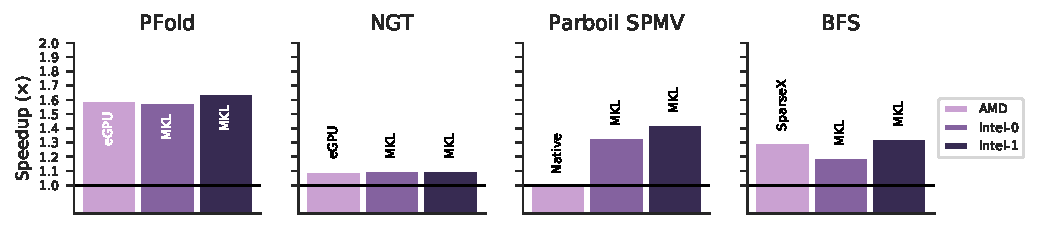
\includegraphics[width=\linewidth]{figures/baseline.pdf}
  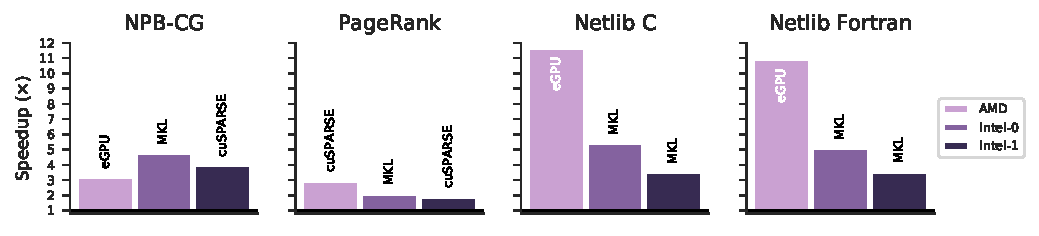
\includegraphics[width=\linewidth]{figures/baseline_bench.pdf}
\\[-0.75em]
  \caption{Evaluation on real-world application code and well-known benchmark
          suites:
           Bars show geometric mean speedup of best-performing LiLAC harness across the
           set of input examples for each benchmark and platform. }
  \label{spmv_app_perf}
\end{figure*}

The speedups that LiLAC achieves on real applications as well as benchmarks are
shown in \autoref{spmv_app_perf}.
They range from $1.1$--$3\times$ on the scientific application codes to
12$\times$ on well-known sparse benchmark programs.

On the \textsc{pathsample} applications (PFold and NGT), we measured
consistent speedups of approximately 50$\%$ and 10$\%$ respectively across
all 3 platforms.
For large applications, Amdahl's law is a severe limitation for
approaches like ours --- other parts of the applications dominate execution
times when linear algebra is accelerated.

PageRank requires a large number of SPMV calls using the same input matrix to
iterate until convergence.
The GPU implementations running on AMD and Intel-1 are able to take advantage of
data remaining in memory.
The larger number of CPU cores and slower GPU available on \mbox{Intel-0} make
MKL its best-performing implementation.
CPU implementations perform best on BFS by avoiding memory copies entirely
--- on AMD, SparseX outperforms GPU implementations.

On standard sparse linear algebra benchmarks, LiLAC achieves speedups of up to
$12\times$.
The impact is independent of the source language, as the C and FORTRAN versions
of the Netlib benchmark demonstrate.
LiLAC is able to achieve consistent, useful speedups across a variety of
hardware configurations.

    \autoref{fig:performance-distribution} demonstrates that achieving good
    performance independent of the hardware platform is no small feat.
    It shows the distribution of speedups on the NPB-CG benchmark across
    different machines, problem sizes and linear algebra implementation.
    More detailed performance data is in \autoref{tab:perf_data}.
    The best-performing implementation varies considerably, depending on
    characteristics of the problem in question.
    No accelerator library performs well reliably, each harness outperforms
    any other harness on some combination of data set and platform.
    clSPARSE on the AMD iGPU is the only harness that is consistently
    outperformed.

\begin{table*}[t]
  \centering
  \footnotesize
  \begin{tabular}{ll|ccc|ccc|ccc|ccc}
    \multirow{2}{*}{\textbf{Platform}} &
    \multirow{2}{*}{\textbf{Implementation}} &
    \multicolumn{3}{c}{\textbf{PFold}} & \multicolumn{3}{c}{\textbf{NGT}} &
    \multicolumn{3}{c}{\textbf{PageRank}} & \multicolumn{3}{c}{\textbf{BFS}} \\[-0.3em]
    & & \hspace{0.8em}L0\hspace{0.8em} & \hspace{0.8em}L1\hspace{0.8em} & \hspace{0.8em}L2\hspace{0.8em}
      & \hspace{0.8em}L0\hspace{0.8em} & \hspace{0.8em}L1\hspace{0.8em} & \hspace{0.8em}L2\hspace{0.8em}
      & \hspace{0.35em}Erdos\hspace{0.35em} & LJ-2008 & \hspace{0.35em}Road\hspace{0.35em}
      & \hspace{0.35em}Erdos\hspace{0.35em} & LJ-2008 & \hspace{0.35em}Road\hspace{0.35em} \\
    \hline
    \hline
    \multirow{3}{*}{Intel-0} 
    & MKL & 2.88 & 2.46 & 1.00 & 1.18 & 1.18 & 1.18 & 1.25 & 2.93 & 1.72 & 2.50 & 1.06 & 1.05 \\[-0.3em]
    & cuSPARSE & 0.75 & 0.60 & 0.45 & 0.66 & 0.66 & 0.66 & 1.39 & 1.00 & 3.32 & 0.87 & 1.74 & 1.28 \\[-0.3em]
    & clSPARSE & 0.90 & 0.75 & 0.46 & 0.81 & 0.79 & 0.78 & 1.24 & 0.95 & 2.24 & 0.13 & 1.45 & 0.07 \\[-0.3em]
    & SparseX & - & - & - & - & - & - & - & - & - & 1.19 & - & - \\
    \hline
    \multirow{3}{*}{Intel-1}
    & MKL & 2.70 & 2.43 & 1.01 & 1.20 & 1.20 & 1.19 & 1.63 & 1.03 & 2.26 & 1.06 & 2.09 & 1.27 \\[-0.3em]
    & cuSPARSE & 0.48 & 0.41 & 0.30 & 0.68 & 0.69 & 0.68 & 1.59 & 0.87 & 4.44 & 1.01 & 1.83 & 1.63 \\[-0.3em]
    & clSPARSE & 1.00 & 1.00 & 1.00 & 1.00 & 1.02 & 1.00 & 1.50 & 0.87 & 3.46 & 0.23 & 1.81 & 0.13 \\[-0.3em]
    & SparseX & - & - & - & - & - & - & - & - & - & 1.25 & - & - \\
    \hline
    \multirow{4}{*}{AMD}
    & cuSPARSE & 1.38 & 1.18 & 0.67 & 0.69 & 0.69 & 0.70 & 3.44 & 1.18 & 9.97 & 1.62 & 6.55 & 1.96 \\[-0.3em]
    & clSPARSE (eGPU) & 2.17 & 1.82 & 1.22 & 1.16 & 1.16 & 1.16 & 3.08 & 1.24 & 6.06 & 0.50 & 11.03 & 0.24 \\[-0.3em]
    & clSPARSE (iGPU) & 2.03 & 1.78 & 1.03 & 0.90 & 0.90 & 0.90 & 3.26 & 1.31 & 4.05 & 0.14 & 4.17 & 0.05 \\[-0.3em]
    & SparseX & - & - & - & - & - & - & - & - & - & 1.93 & - & - \\
  \end{tabular}
\vspace{0.5em}
  \caption{LiLAC speedups on each platform, across different applications and
  problem sizes.
  SparseX demonstrated promising performance on some applications, but we were
  unable to evaluate on every relevant instance due to instability.}
  \label{tab:perf_data}
\vspace{-2em}
\end{table*}

\begin{figure}[t]
  \centering
  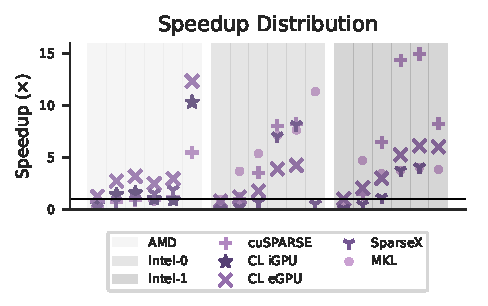
\includegraphics[width=\columnwidth,height=0.67\columnwidth]{figures/distribution.pdf}
\\[-0.75em]
  \caption{Distribution of speedups achieved by LiLAC on the NPB-CG benchmark.
    Each column of points shows the speedup achieved by each implementation
    available on a platform for a particular problem size. Data is sorted along
  the $x$-axis by the best speedup in that column.}
  \label{fig:performance-distribution}
\end{figure}

We verify that LiLAC can reach near-optimal performance, despite using general
and portable harnesses, by comparing the achieved speedups with the performance
of reference implementations.
This was possible on the NPB and Parboil benchmarks, where expert hand
crafted version are available that achieve close to peak performance.


\autoref{tab:lilac-linesofcode} shows our results from these experiments.
For context, we also measure application programmer effort for peak performance,
which is substantial, requiring hundreds of lines of carefully crafted
high performance OpenCL code.
On the NPB-CG benchmark, we achieve $\sim 3\times$ speedup,
while the expert implementation is approximately 3$\times$ faster than LiLAC.
This is partly due to Amdahl's law --- the benchmark also performs operations
other than sparse matrix-vector multiplication and the expert implementation is
a complete rewrite that performs all these operations on the GPU.
On Parboil SPMV, the difference between an expert and LiLAC is only
1.07$\times$.

\begin{figure}[t]
  \centering
  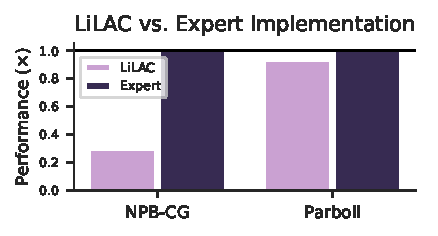
\includegraphics[width=0.9\columnwidth,height=0.5\columnwidth]{figures/expert.pdf}
\\[0.5em]
  \begin{tabular}{lrr}
    \multirow{2}{*}{\textbf{Benchmark}} & \multicolumn{2}{c}{\textbf{Modified LoC}} \\
    & LiLAC & Expert \\
    \toprule
    \toprule
    NPB          & 0 (44) & 1948 \\
    Parboil SPMV & 0 (44) & 261
  \end{tabular}
\\[0.45em]
  \caption{LiLAC vs Expert: We achieve good performance with no application
           programmer effort (measured as required LoC change).
           LiLAC code to be written by library developers is in parentheses.
           Amdahl's Law limits our impact on NPB.
}
  \label{tab:lilac-linesofcode}
\end{figure}

After moving the burden of targeting accelerators from the user to the
library vendor with LiLAC, we would also like to automate the selection of which
library to use.
This may change over time and per application, as we saw in
\autoref{fig:performance-distribution}.
We have experimented with simple classifiers for each platform, that dynamically
select the best library given the data input.
This was straightforward to achieve for our problem space, but more data is
needed for a meaningful evaluation, and we leave it to future work.


\subsection{Effectiveness of Data Marshaling}
Our implementation of LiLAC relies on a non-trivial data marshaling system that
prevents redundant computations and memory transfers. We present performance
results that show the importance and effectiveness of this system.

\begin{figure}[t]
  \centering
  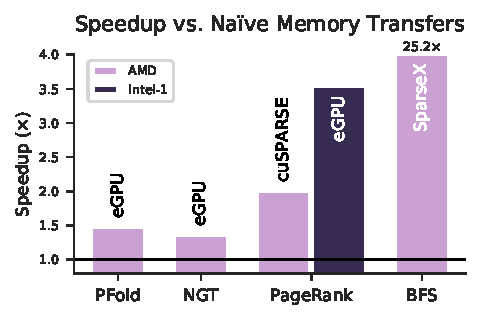
\includegraphics[width=\columnwidth,height=0.67\columnwidth]{figures/marshall.pdf}
\\[-0.75em]
  \caption{LiLAC vs. na\"ive library calls without harnesses.
           Avoiding memory transfers is necessary for performance.}
  \label{fig:transfer-performance}
\end{figure}

We repeated our experiments, using the best-performing implementations from
\autoref{spmv_app_perf}.
Instead of using our data marshaling scheme, we transfer memory naively for
each accelerator invocation.
We then measured the performance advantage that our harness system gives us over
this naive approach, results are in \autoref{fig:transfer-performance}.
The GPU implementations received speedups of 1.4--3.5$\times$ and SparseX was
sped up by over $25\times$ (because it performs an internal matrix tuning phase
that is far more expensive than a memory copy).
These speedups are large enough that in each case, the application would in fact
have performed worse than their sequential baselines without performing data
marshaling.

\begin{table}[b]
\centering
\caption{Sparsity does not fit the polyhedral model, Intel compilers fail to
         parallelize and Polly is not available for FORTRAN.
         Only LiLAC detects sparse linear algebra reliably.}
\label{compareiccpolly}
\vspace{-0.5em}
\small
\begin{tabular}{l|c|c|c}
{\bf Benchmark}      & {\bf LiLAC}    & {\bf Polly}   & {\bf Intel icc/ifort} \\
\hline
\hline
PFold          & CSR & - & parallel dependence \\[-0.3em]
NGT            & CSR & - & parallel dependence \\[-0.3em]
Parboil-SPMV   & JDS & no SCoP & parallel dependence \\[-0.3em]
BFS            & CSR & no SCoP & parallel dependence \\[-0.3em]
NPB-CG         & CSR & - & parallel dependence \\[-0.3em]
PageRank       & CSR & no SCoP & parallel dependence \\[-0.3em]
Netlib C       & CSR & no SCoP & parallel dependence \\[-0.3em]
Netlib Fortran & CSR & - & parallel dependence \\
\end{tabular}
\end{table}

\subsection{Reliability of Discovery}

    To achieve performance impact, LiLAC needs to reliably detect linear algebra
    computations, independent of coding style and source programming language.
    The results so far demonstrated that this works reliably and the data in
    \autoref{compareiccpolly} reiterates this.
    Established approaches, like the polyhedral model, on the otehr hand, are
    unable to model sparse linear algebra.
    We verified this with the Polly compiler and found that no SCoPs captured
    sparse linear algebra.
    This is unsurprising, as the basic assumptions of affine memory access are
    contradicted by the indirection that is inherent in sparsity.
    Similarly, the Intel icc and ifort compilers fail to auto-parallelize, as
    they cannot reason about sparsity and have to assume additional dependencies
    where sparse accesses occur.


\section{Conclusion}
\label{sec:conclusion}
% Sparse and dense linear algebra are critical workloads for many important
% established applications and will only gain more significance with emerging
% domains such as deep learning and AI.

% Past experience has shown that acceleration solutions that require even limited
% modifications of legacy source code hinder mainstream adoption.
% Hence, the providion of custom APIs for new accelerator hardware is insufficient
% to penetrate scientific computing outside of elite projects.
% At the same time, entirely compiler based solution have failed to scale and
% perform.

% We have demonstrated that our approach of compiler based detection coupled with
% library based acceleration manages to combine the advantages of both, achieving
% the full performance without requiring programmer intervention.
% We showed that this scales to large scientific codes across multiple programming
% languages.

This paper has presented LiLAC, a language and compiler that enables existing
code bases to exploit sparse (and dense) linear algebra accelerator libraries.
No effort is required from the application programmer.
Instead, the library implementer provides a few lines of specification, which
LiLAC uses to  automatically and efficiently matches  user code to
underlying high performance libraries.

We demonstrated this approach on  C, C++ and FORTRAN benchmarks as well as
legacy applications and shown significant performance improvement across
platforms and data sets.
Many language features of the LiLAC language could be repurposed for libraries
beyond linear algebra.
In future work, we will investigate how our framework could be adapted to other
application domains, enabling effort free access to an even larger set of
accelerator libraries.

